\documentclass{article}
\usepackage[T1]{fontenc}
\usepackage[utf8]{inputenc}

\usepackage{color}
\usepackage{tikz}
%\usetikzlibrary{}
\usepackage{pgfplots}

\begin{document}

\begin{figure}
    \centering
    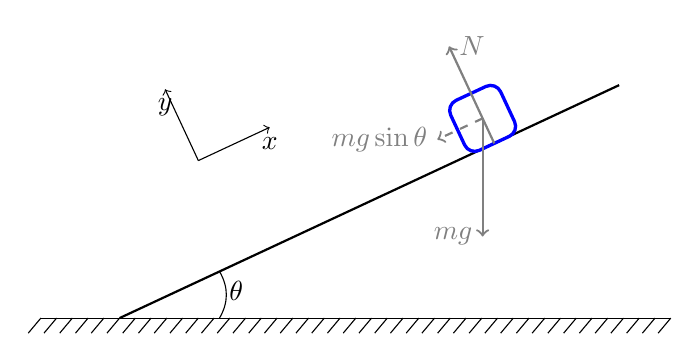
\begin{tikzpicture}
        \def\angle{25}
        \def\size{0.7}
        \def\force{1.5}
        \coordinate (P) at (0,0);

        %Ground
        \draw (P) ++(-1,0) -- +(8,0);
        \draw[thick] (P) -- +(\angle:7) coordinate[pos=0.2] (A) coordinate[pos=0.7] (B);
        \draw (A |- P) to[bend right] (A.center);
        \node[below right] at (A) {$\theta$};
        \foreach \x in {-1,-0.8,...,7}{
            \draw[thin] (\x,0) -- +(-130:0.25);
        }

        %Axis
        \draw[->] (P) ++(1,2) -- +(\angle:1) node[pos=1,below]{$x$};
        \draw[->] (P) ++(1,2) -- +(90+\angle:1) node[pos=1,below]{$y$};

        %Box
        \draw[blue, very thick, rounded corners, rotate around={\angle:(B)}] (B) rectangle +(\size,\size);
        \path (B) -- ++(\angle:0.5*\size) coordinate[pos=1] (Y) -- +(90+\angle:0.5*\size) coordinate[pos=1] (Z);

        %Vectors
        \draw[gray, thick, ->] (Z.center) -- +(0,-\force) node[pos=1,left]{$mg$};
        \draw[dashed, gray, thick, ->] (Z.center) -- +(180+\angle:{\force*sin(\angle)}) node[pos=1,left]{$mg\sin\theta$};
        \draw[gray, thick, ->] (Y.center) -- +(90+\angle:{\force*cos(\angle)}) node[pos=1,right]{$N$};
    \end{tikzpicture}
    \label{}
    \caption{}
\end{figure}


\begin{tikzpicture}
    \begin{axis}[xlabel=$x$, ylabel=$y$]
        \addplot[variable=\x,domain=0:10,samples=100] {sin(deg(\x))};
        \addplot[red,thick] table {data.txt}; %Avhengig av filen data.txt i samme mappe
    \end{axis}
\end{tikzpicture}


\end{document}
